\documentclass[4paper]{article}
\usepackage[spanish]{babel}
%\usepackage[ansinew]{inputenc}
\usepackage[utf8x]{inputenc}
%\usepackage[utf-8]{inputenc}
%\usepackage[T1]{fontenc}
\usepackage{graphicx}
\usepackage{multicol}
%\usepackage{longtable}
%\usepackage{array}
%\usepackage{multirow}
%\usepackage[latin1]{inputenc}
%\inputencoding{latin1}

\renewcommand{\tablename}{Tabla}
\author{Manuel Molino Milla \and Luis Molina Garzón}
\title{\textbf{Polimorfismo}
\\Cadenas}
\date{\today}
\begin{document}

\maketitle

\subsection*{Ejercicio 1}
Crea una clase abstracta denominada \emph{PoligonoRegular} que contenga:
\begin{itemize}
\item Tres campos que especifiquen el nombre del polígono, el número de lados y la longitud del lado.
\item El constructor correspondiente.
\item Un método que devuelva el perímetro de dicho poligono regular.
\item Un método abstracto para definir el área del polígono.
\item Un método \emph{toString()} que devuelva el nombre del polígono y la longitud del lado.
\item Sobrescribe el método \emph{equals} y nos diga que dos polígonos son iguales si tienes el mismo número de lados y la longitud del lado es la misma. \emph{Hay que sobrescribir el método, no sobrecargarlo}.
\item Define el método \emph{compareTo} de la interfaz \emph{Comparable} para que cuando compare dos poligonos regulares nos de la diferencia de lados entre ellos.
\end{itemize}
Crea posteriormente tres clases denominadas \emph{TrianguloEquilatero, Cuadrado y Hexagono} que hereden de la clase PoligonoRegular. Recuerda que deben escribir el método abstracto para el calcular el área.\\
Crea una clase \emph{ListaPoligonoRegular} que sea una \emph{composición} de objetos de tipo \emph{PoligonoRegular}\\
Crea una clase denominada \emph{TestPoligonoRegular} que haga lo siguiente:
\begin{itemize}
\item Cree tres triangulos rectángulos, tres cuadrados y tres hexágonos. 
\item Guardalos en un objeto de tipo \emph{ListaPoligonoRegulares}.
\item Recorriendo la lista de polígonos debes invocar al método \emph{toString()} para que informe de que tipo de poligono es e indique ademas el valor de su perímetro y de su área.
\item Vuelve a recorrer la lista para comprobar que objeto es igual al primero  usando el método \emph{equals}
\item Idem pero usando el método \emph{compareTo()}.
\end{itemize}
Realiza el correspondiente diagrama UML.
\newpage
\subsection*{Ejercicio 2}
Usando el diagrama UML, implementa las clases correspondientes y realiza una clase Test que compruebe el correcto funcionamiento.
\\ 
\vspace*{0.2cm}
\begin{figure}[h]
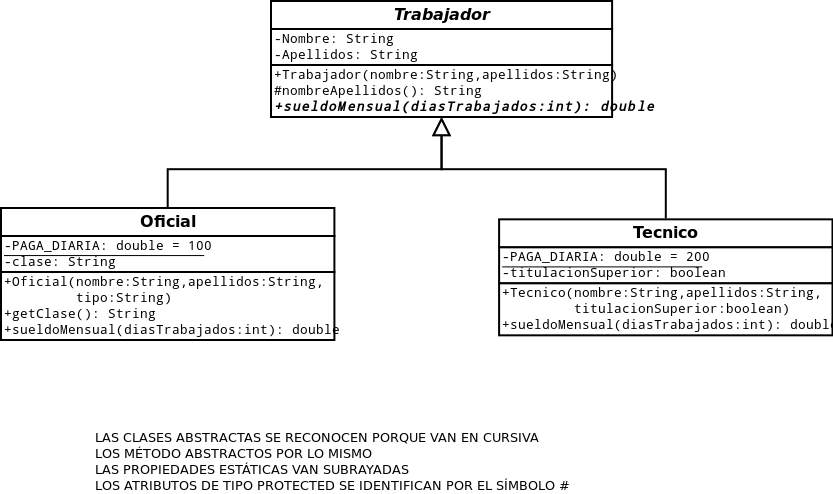
\includegraphics[scale=0.4]{herencia.png}
\end{figure}
\\ 
\vspace*{0.2cm}

\newpage
\subsection*{Ejercicio 3}
Usando el diagrama UML implementa las clases que se piden. En el método \emph{acelerar y frenar} debe devolver una referencia de texto (coche o moto) mas la velocidad actual del vehículo. En el caso que se supere la velocidad máxima también se debe alertar.
\\ 
Implementa una clase Test que compruebe el correcto funcionamiento.
\vspace*{0.2cm}
\begin{figure}[h]
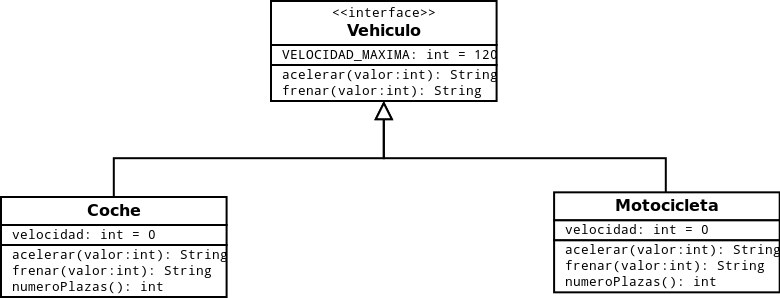
\includegraphics[scale=0.4]{interfaces.png}
\end{figure}
\\ 
\vspace*{0.2cm}
\subsection*{Ejercicio 4}
Construir una clase \emph{ArrayReales} que declare un atributo de tipo \emph{double[]} y que implemente una interfaz llamada \emph{Estadisticas}. El contenido de esta interfaz es el siguiente:
\begin{verbatim}
public interface Estadisticas {
   double minimo();
   double maximo();
   double sumatorio();
}
\end{verbatim}

\subsection*{Ejercicio 5}
Construir una clase \emph{final Math3} que amplíe las declaraciones de métodos estáticos de la clase \emph{Math} y que implemente una interfaz llamada \emph{Extremos} compilada con el siguiente código fuente.
\begin{verbatim}
public interface Extremos{
  int min(int [] a);
  int max(int [] a);
  double min(double [] a);
  double max(double [] a);
}
\end{verbatim}

\end{document}
